\documentclass[a4paper,12pt]{article}
\usepackage{graphicx} % For images
\usepackage{hyperref} % For hyperlinks
\usepackage{amsmath} % For math symbols
\usepackage{listings} % For code snippets
\usepackage{xcolor} % For custom colors in code
\usepackage{geometry} % To change the page layout
\geometry{margin=1in}
\usepackage[french]{babel} % For French language support

% Define custom colors for code
\definecolor{codegray}{rgb}{0.5,0.5,0.5}
\definecolor{codepurple}{rgb}{0.58,0,0.82}
\definecolor{backcolour}{rgb}{0.95,0.95,0.92}

% Set up code formatting style
\lstdefinestyle{mystyle}{
    backgroundcolor=\color{backcolour},
    commentstyle=\color{codegray},
    keywordstyle=\color{codepurple},
    numberstyle=\tiny\color{codegray},
    stringstyle=\color{red},
    basicstyle=\ttfamily\footnotesize,
    breakatwhitespace=false,
    breaklines=true,
    captionpos=b,
    keepspaces=true,
    numbers=left,
    numbersep=5pt,
    showspaces=false,
    showstringspaces=false,
    showtabs=false,
    tabsize=2
}
\lstset{style=mystyle}

\title{UE : Networks : Connected and secure\\ \textbf{Cybersécurité 1 (documentation)}}
\author{Mattias Bruneau, Augustin Vangeebergen}
\date{\today}

\begin{document}

\maketitle
\begin{figure}[h]
\centering

\includegraphics[width=0.5\textwidth]{logo.png}
\label{fig:logoheh}
\end{figure}
\newpage

\tableofcontents
\newpage
\section{Informations générales}
\begin{itemize}
    \item Nom du projet : Gestion et sécurisation d'une agence Cyber Sécurité
    \item Date de début : 24/09
    \item Local : 2.16
    \item Responsable : Bruneau Mattias, VanGeebergen Augustin Agence 7
    \item Équipements utilisés : Cisco Router, Cisco Pare-feu, Cisco Switch 
    \item Objectif : Créer et sécuriser une infrastructure réseau
\end{itemize}

\subsection{FW}
\begin{itemize}
\item Modèle: FortiGate 60E
\item Firmware: v7.4.3 build2573
\item Hostname: AG\_7\_FW\_1\_PD\_P
\item Serial number: FGT60ETK1809A3ED
\end{itemize}
\subsection{Routeur}
\begin{itemize}
\item Modèle : C8200L-1N-4T
\item Hostname : AG\_7\_RT\_1\_PD\_P
\end{itemize}
\subsection{Switch}
\begin{itemize}
\item Modèle : C1000-24T-4G-L V01
\item Hostname : AG\_7\_SW\_1\_PD\_P
\end{itemize}
\newpage
\section{Topologies}
\subsection{Topologie globale}
Voir annexe 1 : Topologie Globale
\subsection{Topologie locale de l'agence 7}
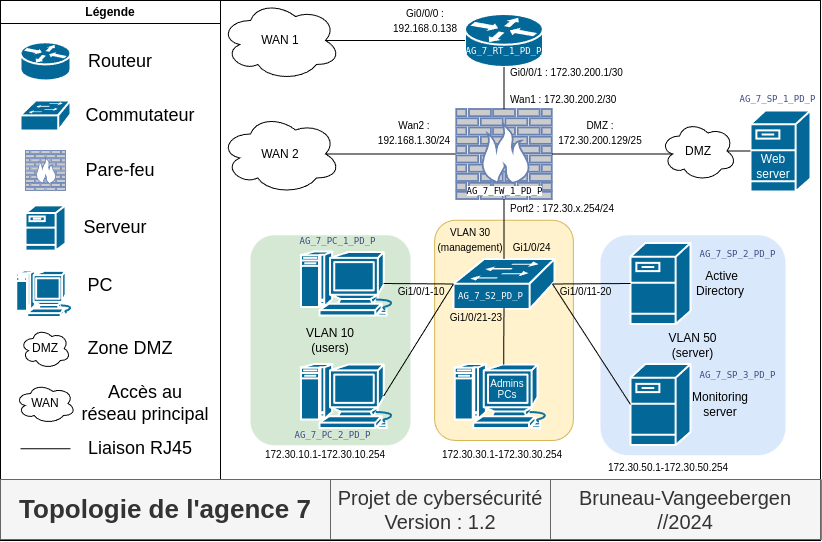
\includegraphics[width=1\textwidth]{topo_locale.png}

\newpage


\subsection{[25/09]}

\subsubsection{Firewall}

\begin{itemize}
\item Apres firewall reset : interface 1 utilisée pour se connecter à la WebUI.
\item Adresse : 192.168.1.99/255.255.255.0
\item Mot de passe du compte "admin" : @0Test123*
\end{itemize}


\subsubsection{Routeur}

\begin{itemize}
\item Connexion pour la première fois au routeur apres reset, choisir "skip initial installation"
\item MDP acces console et mode privilégié : @0Test123*
\end{itemize}

\subsubsection{Switch}

\begin{itemize}
\item Connexion pour la première fois au switch apres reset, choisir "skip initial installation"
\item MDP acces console et mode privilégié : @0Test123*
\end{itemize}


\subsubsection{Problèmes rencontrés}
\begin{itemize}
\item Problème d'affichage dans le terminal (il suffit d'appuyer plsieurs fois sur enter).
\end{itemize} 


\newpage


\subsection{[02/10]}



\subsubsection{Router}

\begin{itemize}
\item Gestion des interfaces (IP Statiques WAN1, FW)
\item Assignation WEB ui
\end{itemize} 


\subsubsection{Firewall}

\begin{itemize}
\item Création des interfaces pour les VLANs (sous-interfaces avec assignations des ranges IP en DHCP)
\end{itemize} 
\subsubsection{Switch}

\begin{itemize}
\item Gestion des VLANs + assignations des ports
\end{itemize} 
\subsubsection{Problèmes rencontrés}
\begin{itemize}
\item Pas de problèmes majeurs rencontrés. (Temps de réponse FW)
\end{itemize} 
\subsubsection{Planification des tâches pour le cours suivant}
\begin{itemize}
\item Router : Gestion SSH + Banner motd + Timeout après 3 essais et après 5 min d'inactivité
\item Firewall : Création interface DMZ + Création interface WAN2 + assignation des adresses IP statiques + Banner motd + Timeout après 3 essais et après 5 min d'inactivité
\item Switch : Banner motd + SSH + Timeout après 3 essais et après 5 min d'inactivité
\end{itemize} 

\newpage


\subsection{[03/10]}

\subsubsection{Router}

\begin{itemize}

\item SSH + banner + timeout
\end{itemize} 

\subsubsection{Firewall}


\begin{itemize}

\item DMZ + WAN 2 + IP statiques DMZ et WAN 2 + banner + timeout
\end{itemize} 

\subsubsection{Switch}

\begin{itemize}

\item SSH + banner + timeout
\end{itemize} 

\subsubsection{Problèmes rencontrés}
\begin{itemize}

\item Problème SSH sur le switch étant donné mauvaise version IOS

\end{itemize} 

\subsubsection{Planification des tâches pour le cours suivant}
\begin{itemize}


\item Router : Ajout de sécurité lié au ssh (TO, Logging events, retries)
\item Firewall : règles fw (création de policies) + port sécurity + dhcp snooping
\item Switch : Ajout de sécurité lié au ssh (TO, Logging events, retries)
\end{itemize} 

\newpage
\subsection{[07/10]}

\subsubsection{Router}

\begin{itemize}

\item Vérification device (SSH, sécurité) + ajout des sécurités SSH
\end{itemize} 

\subsubsection{Firewall}

\begin{itemize}

\item Création des règles du FW (policies), port security, dhcp snooping

\end{itemize} 
\subsubsection{Switch}

\begin{itemize}

\item Vérification device (SSH, sécurité) + ajout des sécurités SSH
\end{itemize} 
\subsubsection{Problèmes rencontrés}
\begin{itemize}

\item /
\end{itemize} 
\subsubsection{Planification des tâches pour le cours suivant}
\begin{itemize}

\item Router : Vérification apr le professeur de nos configurations
\item Firewall : Vérification apr le professeur de nos configurations
\item Switch : Vérification apr le professeur de nos configurations


\end{itemize} 

\section{Troubleshooting}
% Add your troubleshooting information here

\section{Sources}
% Add your sources here
\section{Annexes}
\subsection{Topologie globale}
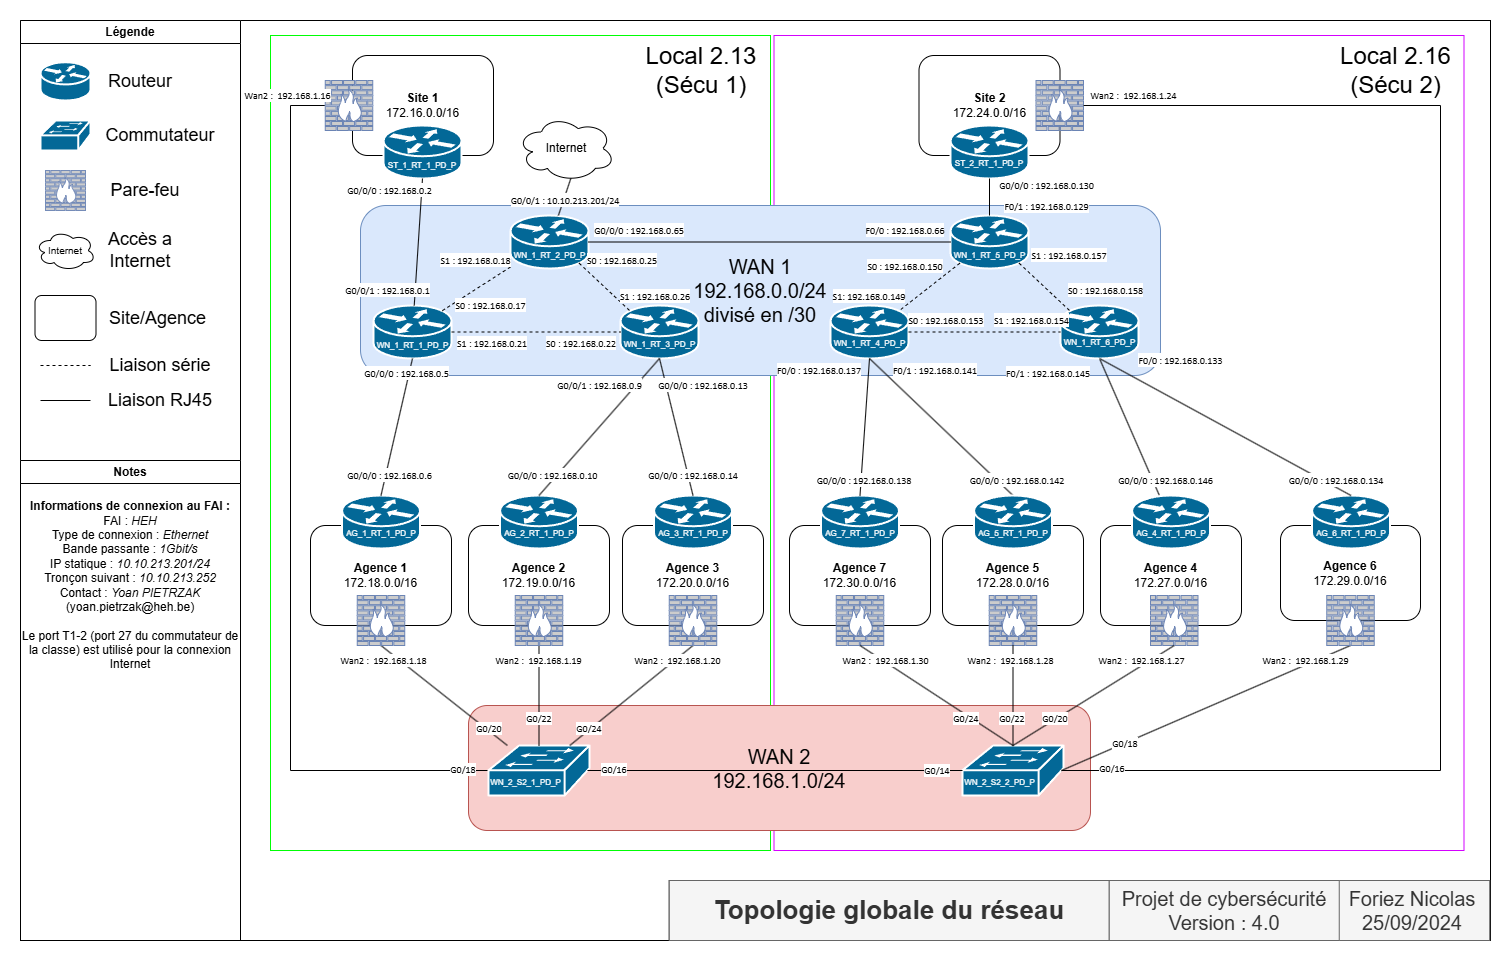
\includegraphics[width=1\textwidth]{topo_globale.png}

\end{document}
